\documentclass{article}

\usepackage[a4paper]{geometry}
\usepackage[utf8]{inputenc}
\usepackage[colorlinks=false]{hyperref}
\usepackage{verbatim}

\usepackage{graphicx}
\graphicspath{ {./resources/} }
\usepackage{titlesec}

% Todo list
\usepackage{enumitem, amssymb}
\newlist{todolist}{itemize}{2}
\setlist[todolist]{label=$\square$}
\usepackage{pifont}
\newcommand{\cmark}{\ding{51}}%
\newcommand{\xmark}{\ding{55}}%
\newcommand{\done}{\rlap{$\square$}{\raisebox{2pt}{\large\hspace{1pt}\cmark}}%
\hspace{-2.5pt}}
\newcommand{\wontfix}{\rlap{$\square$}{\large\hspace{1pt}\xmark}}

% Blue linked files blocks.
\usepackage{framed, color}
\definecolor{shadecolor}{RGB}{230, 247, 255}

% Gray Code blocks.
\usepackage{listings}
\definecolor{codeBG}{gray}{0.80}
\lstset{
  backgroundcolor=\color{codeBG},
  frame=single,
  basicstyle=\fontsize{9}{11}\selectfont\ttfamily,
  columns=fullflexible,
  breaklines=true,
  keepspaces=true,
  title=\lstname
  }

\title{Aantekeningen automatisch onderwerpsontsluiting ebooks m.b.v. Annif}
\author{Thomas Haighton}

\begin{document}

\maketitle

\clearpage

\tableofcontents

\clearpage

\section{Inleiding}
Dit document bevat mijn aantekeningen m.b.t. het testen van Annif t.b.v. het automatisch toekennen van onderwerpen aan E-books binnen de KB. 

De KB hanteert een eigen classificatiesysteem/thesaurus genaamd Brinkman catalogus. Op de \href{https://www.kb.nl/bronnen-zoekwijzers/zoekwijzers/meer-informatie-over-zoeken/trefwoorden-in-de-kb-catalogus}{KB website} is meer informatie te vinden m.b.t. de verschillende trefwoordcatalogi binnen de KB.

Bij aanvang van dit onderzoek was er sprake van een mogelijke samenwerking tussen de KB en het \href{https://www.cb.nl}{CB}. Waar de KB de onderwerpen vastlegt d.m.v. Brinkmantrefwoorden, werkt het CB met \href{https://www.editeur.org/151/Thema/}{Thema}.

\section{Data}

\subsection{Overeenkomsten Thema en Brinkman}

Het eerste onderzoek was gericht op het vinden van overeenkomsten tussen de brinkmanonderwerpen en de onderwerpen zoals deze stonden vastgelegd in Thema. Bij de vergelijking zijn alle termen eerst geconverteerd naar kleine letters (lowercase), omdat Thema onderwerpen altijd beginnen met een hoofdletter en in Brinkman alleen trefwoorden zoals plaatsnamen of persoonsnamen met een hoofdletter beginnen.
\\

\begin{tabular}{|l|l|l|}
\hline
\_                    & Brinkman  & Thema \\
\hline
Totaal aantal termen  & 14737     & 7362 \\
Unieke termen         & 13729     & 6355 \\
Overeenkomende termen & 980       & \_   \\
\hline
\end{tabular}

% TODO: discrepantie (zou 1008 moeten zijn?)

Zie \href{https://github.com/KBNLresearch/Annif_data_exp/blob/master/compare_Brinkman_and_Thema.ipynb}{Jupyter Notebook op GitHub}\\[2pt]

\noindent
\textit{Constatering} \\
Als we kijken naar een trefwoord wat alleen in Brinkman voorkomt, maar waarvan we verwachten dat deze ook in Thema zou moeten staan, b.v. 'autisme'. In Thema wordt 'autisme' vastgelegd in 'autisme en asperger syndroom'en 'omgaan met autisme/asperger'. Het zou dus mogelijk zijn dat er meer overlap mogelijk is.

N.B.: Het CB heeft laten weten (tijdelijk) af te zien van dit project. Verder onderzoek met Thema is na dit bericht gestaakt en is er alleen gekeken naar Brinkmantrefwoorden.


\subsection{GGC dataset}

De gebruikte dataset is een query aan het GGC als TSV (Tab Seperated Values) tekst bestand. De query bestaat uit verschillende eisen:

\begin{itemize}
    \item Is een e-book
    \item Jaar van uitgave is tussen 2015-2019
    \item Nederlandstalig
    \item Er is minimaal één Brinkman-trefwoord toegekend
    \item Samenvattingsveld (KMC 4207) is niet leeg
\end{itemize}

De verkregen dataset bevat 12243 regels.

\begin{shaded}
Bekijk de sql query: \quad
\href{run:resources/ggc_query.sql}{\textbf{\textit{ggc\_query.sql}}}

Bekijk de output: \quad \quad
\href{run:resources/vraag_20190620.txt}{\textbf{\textit{vraag\_20190620.txt}}}
\end{shaded}

Tot nu toe zijn hier 3 verschillende datasets mee gemaakt, elk gesplits in een train (15\%), eval (5\%) en test set (80\%). 
\begin{itemize}
  \item ggc1.zip: bevat alleen samenvattingen/flaptekst van alle E-books.
  \item ggc2.zip: bevat titel, ondertitel (wanneer deze aanwezig is) en samenvatting/flaptekst van alle E-books.
  \item ggc3.zip: bevat titel, ondertitel (wanneer deze aanwezig is) en samenvatting/flaptekst van E-books die geen vormtrefwoorden hebben toegekend.
\end{itemize}

\textbf{Top 20 meest toegewezen Brinkmantrefwoorden}


\begin{tabular}{| l | l | l |}
\hline
\textbf{index} & \textbf{Toegewezen Brinkmantrefwoorden} & \textbf{Aantal x toegewezen} \\
\hline
0  &           romans en novellen ; vertaald                       &  2165  \\
1  &           romans en novellen ; oorspr. - Nederlands           &  1960  \\
2  &                              jeugdboeken ; verhalen           &  1265  \\
3  &                                levensbeschrijvingen           &  193   \\
4  &                    gedichten ; oorspr. - Nederlands           &  181   \\
5  &                                    autobiografieën            &  99    \\
6  &                                             columns           &  61    \\
7  &                                         levenskunst           &  55    \\
8  &                                       stripverhalen           &  48    \\
9  &              jeugdboeken ; verhalen | prentenboeken           &  46    \\ 
10 &                                       geloofsleven            &  41    \\
11 &  jeugdboeken ; verhalen | romans en novellen ; ...            &  39    \\
12 &                jeugdboeken ; informatie - biologie            &  35    \\
13 &                                      overdenkingen            &  34    \\
14 &             prentenboeken | jeugdboeken ; verhalen            &  34    \\
15 &                                            voetbal            &  33    \\
16 &                                     spiritualiteit            &  33    \\
17 &                                             essays            &  29    \\
18 &                                       leidinggeven            &  26    \\
19 &                                       reisverhalen            &  25    \\
\hline
\end{tabular}

\subsection{Vorm- en Zaaktrefwoorden}
TODO:

\section{Annif}

Annif homepage: \url{http://annif.org/}

\subsection{Train en Evalueer Annif model (in vogelvlucht)}

\href{https://github.com/NatLibFi/Annif/wiki/Getting-started}{Officiele \textit{Getting Started} documentatie}

Ik gebruik /Annif/tests als project map; zoals in de documentatie wordt aangeraden.\\*

Annif commands/options help: \texttt{annif --help}

\begin{enumerate}
  \item (optioneel) Maak eerst een configuratie in \textit{projects.cfg}
  \item Start Annif Python virtual environment (annif-venv), in annif-venv/bin: \texttt{source activate}
  \item Navigeer naar project folder (e.g. Desktop/Annif/Annif/tests) en start Annif: \texttt{annif}
  \item Check of \textit{projects.cfg} gevonden wordt: \texttt{annif list-projects}
  \item Laad onderwerpen: \verb|annif loadvoc PROJECT_ID [SUBJECT_FILE]|
  \item Train model: \verb|annif train PROJECT_ID [PATHS]|
  \item Evalueer model: \verb|annif eval PROJECT_ID [PATHS]|
  \item Gebruik de getrainde modellen (zie H. 3.5)
\end{enumerate}


\subsection{Configuratie}

Voorbeeld Annif configuratie en bijbehorende evaluatie.\\*[1pt]

\noindent
\textbf{TF-IDF backend met snowball analyzer}

\begin{lstlisting}
[tfidf-brinkman]                # PROJECT_ID
name=TF-IDF Brinkman            # Uitgebreidde naam
language=nl                     # Taal
backend=tfidf                   # Backend (algoritme)
analyzer=snowball(dutch)        # Analyzer (stemmer)
limit=100                       # Aantal onderwerpen 
vocab=brinkmanthesaurus_vocab   # Thesaurus
\end{lstlisting}

\subsection{Evaluatie}

\begin{lstlisting}
Precision (doc avg):	0.07161500815660683
Recall (doc avg):   	0.6252039151712887
F1 score (doc avg): 	0.12716049583912553
Precision (conc avg):	0.0033237931737672725
Recall (conc avg):  	0.006049485486600793
F1 score (conc avg):	0.003495638750427632
Precision (microavg):	0.07161500815660685
Recall (microavg):  	0.5480649188514357
F1 score (microavg):	0.12667724715048334
NDCG:               	0.4647151156485022
NDCG@5:             	0.44466032224552277
NDCG@10:            	0.4647151156485022
Precision@1:        	0.29853181076672103
Precision@3:        	0.18651441000543773
Precision@5:        	0.12854812398042414
LRAP:               	0.39799930172762893
True positives:     	439
False positives:    	5691
False negatives:    	362
Documents evaluated:	613
\end{lstlisting}


\noindent
\textbf{Alle evaluatie uitkomsten} \\
Ik heb tot nu toe de volgende backends getest: \textit{TF-IDF, Fasttext, Ensemble van de twee, en Omikuji}. Daarnaast ook kort de twee verschillende analyzers geprobeerd: \textit{snowball} en \textit{simple}. Bij de twee verschillende analyzers heeft de snowball analyzer een hogere score, dus voor de volgende experimenten zal ik alleen nog deze gebruiken. \\
\begin{shaded}
Voor alle uitkomsten van de verschillende configuraties zie: \href{https://github.com/KBNLresearch/Annif_data_exp/blob/master/annif_uitkomsten.xlsx}{\textbf{\textit{annif\_uitkomsten.xlsx}}}
\end{shaded}

%TODO: Na het testen van ggc2 dataset, uitkomsten toevoegen (heeft het toevoegen van (sub)titel een beter uitkomst?).

\subsection{Experimenten}
In onderstaand experiment heb ik gebruik gemaakt van het project \texttt{tfidf-brinkman}.

\subsubsection{Experiment 1} 

Test Annif via command-line interface: \texttt{cat document.txt | annif suggest tfidf-brinkman}

Annif suggestie voor bijbehorende Brinkman termen voor 420818715.txt:

\begin{lstlisting}
cat ./data/Annif-corpora/fulltext/ggc/dev/420818715.txt | annif suggest tfidf-brinkman

<http://data.bibliotheken.nl/id/thes/p075660849>	levenskunst	0.4163530829438607
<http://data.bibliotheken.nl/id/thes/p075665689>	zelfkennis	0.39504628028213046
<http://data.bibliotheken.nl/id/thes/p075606178>	filosofie	0.3769179576596768
<http://data.bibliotheken.nl/id/thes/p075607050>	geloofsleven	0.3712595743673854
<http://data.bibliotheken.nl/id/thes/p07561765X>	organisatieontwikkeling	0.3698668389205731
<http://data.bibliotheken.nl/id/thes/p075663910>	spiritualiteit	0.36965842850694486
<http://data.bibliotheken.nl/id/thes/p075660822>	leidinggeven	0.36507826867675164
<http://data.bibliotheken.nl/id/thes/p075617846>	overdenkingen	0.36310030904972374
<http://data.bibliotheken.nl/id/thes/p075603578>	cultuurfilosofie	0.3629843846776753
<http://data.bibliotheken.nl/id/thes/p075610744>	jeugdboeken ; verhalen	0.36280384270411503
\end{lstlisting}

Daadwerkelijk toegekende Brinkman termen - 420818715.tsv:

\begin{lstlisting}
cat ./data/Annif-corpora/fulltext/ggc/dev/420818715.tsv

<http://data.bibliotheken.nl/id/thes/p075600447>	bedrijfsorganisatie
<http://data.bibliotheken.nl/id/thes/p075603012>	citatenverzamelingen
\end{lstlisting}


Volledige tekst 420818715.txt:

\begin{lstlisting}
cat ./data/Annif-corpora/fulltext/ggc/dev/420818715.txt

Er wordt wat afgeklooid in onze bedrijven en organisaties. Tijd om te ontklooien, dus! Hoe graag zouden we luid gillend willen protesteren tegen alle ellende? We blijken namelijk slechts 15% van onze tijd bezig te zijn met het creëren van waarde. Er zijn tienduizenden bullshitjobs. 75% van alle (ict-)projecten halen hun budget, balance, alsof werken geen leven is. En wat al niet meer... De trieste waarheid is dat werken inderdaad vaak geen leven is. Maar luidop protesteren is een niet zo erg carrièrebevorderende actie. Durven we onze mond dus wel open te doen? Waarschijnlijk niet... Dit boekje snelt u ter hulp. Honderd en een citaten van bekende en minder bekende managementexperts, filosofen en wetenschappers die hun flink gepekelde vinger in de open wonden leggen. Ze vertellen precies wat u en ik denken. We kunnen ermee uitpakken: op ons whiteboard, in een mailtje of anoniem in de kantine. En wij blijven buiten schot, want de goeroe heeft het gedaan. Liever op de achtergrond blijven? Dan hebt u vast veel gniffelplezier bij het lezen van dit boekje. Bent u zelf leidinggevende, manager of directeur? Zoals de Vlaamse dichteres Alice Nahon schreef: 't is goed in 't eigen hart te kijken, des avonds voor het slapengaan. May the force be with you! Bron: Flaptekst, uitgeversinformatie
\end{lstlisting}

\noindent
Test annif als web applicatie: \texttt{annif run} \\
Open in browser: \url{http://localhost:5000/}

\noindent
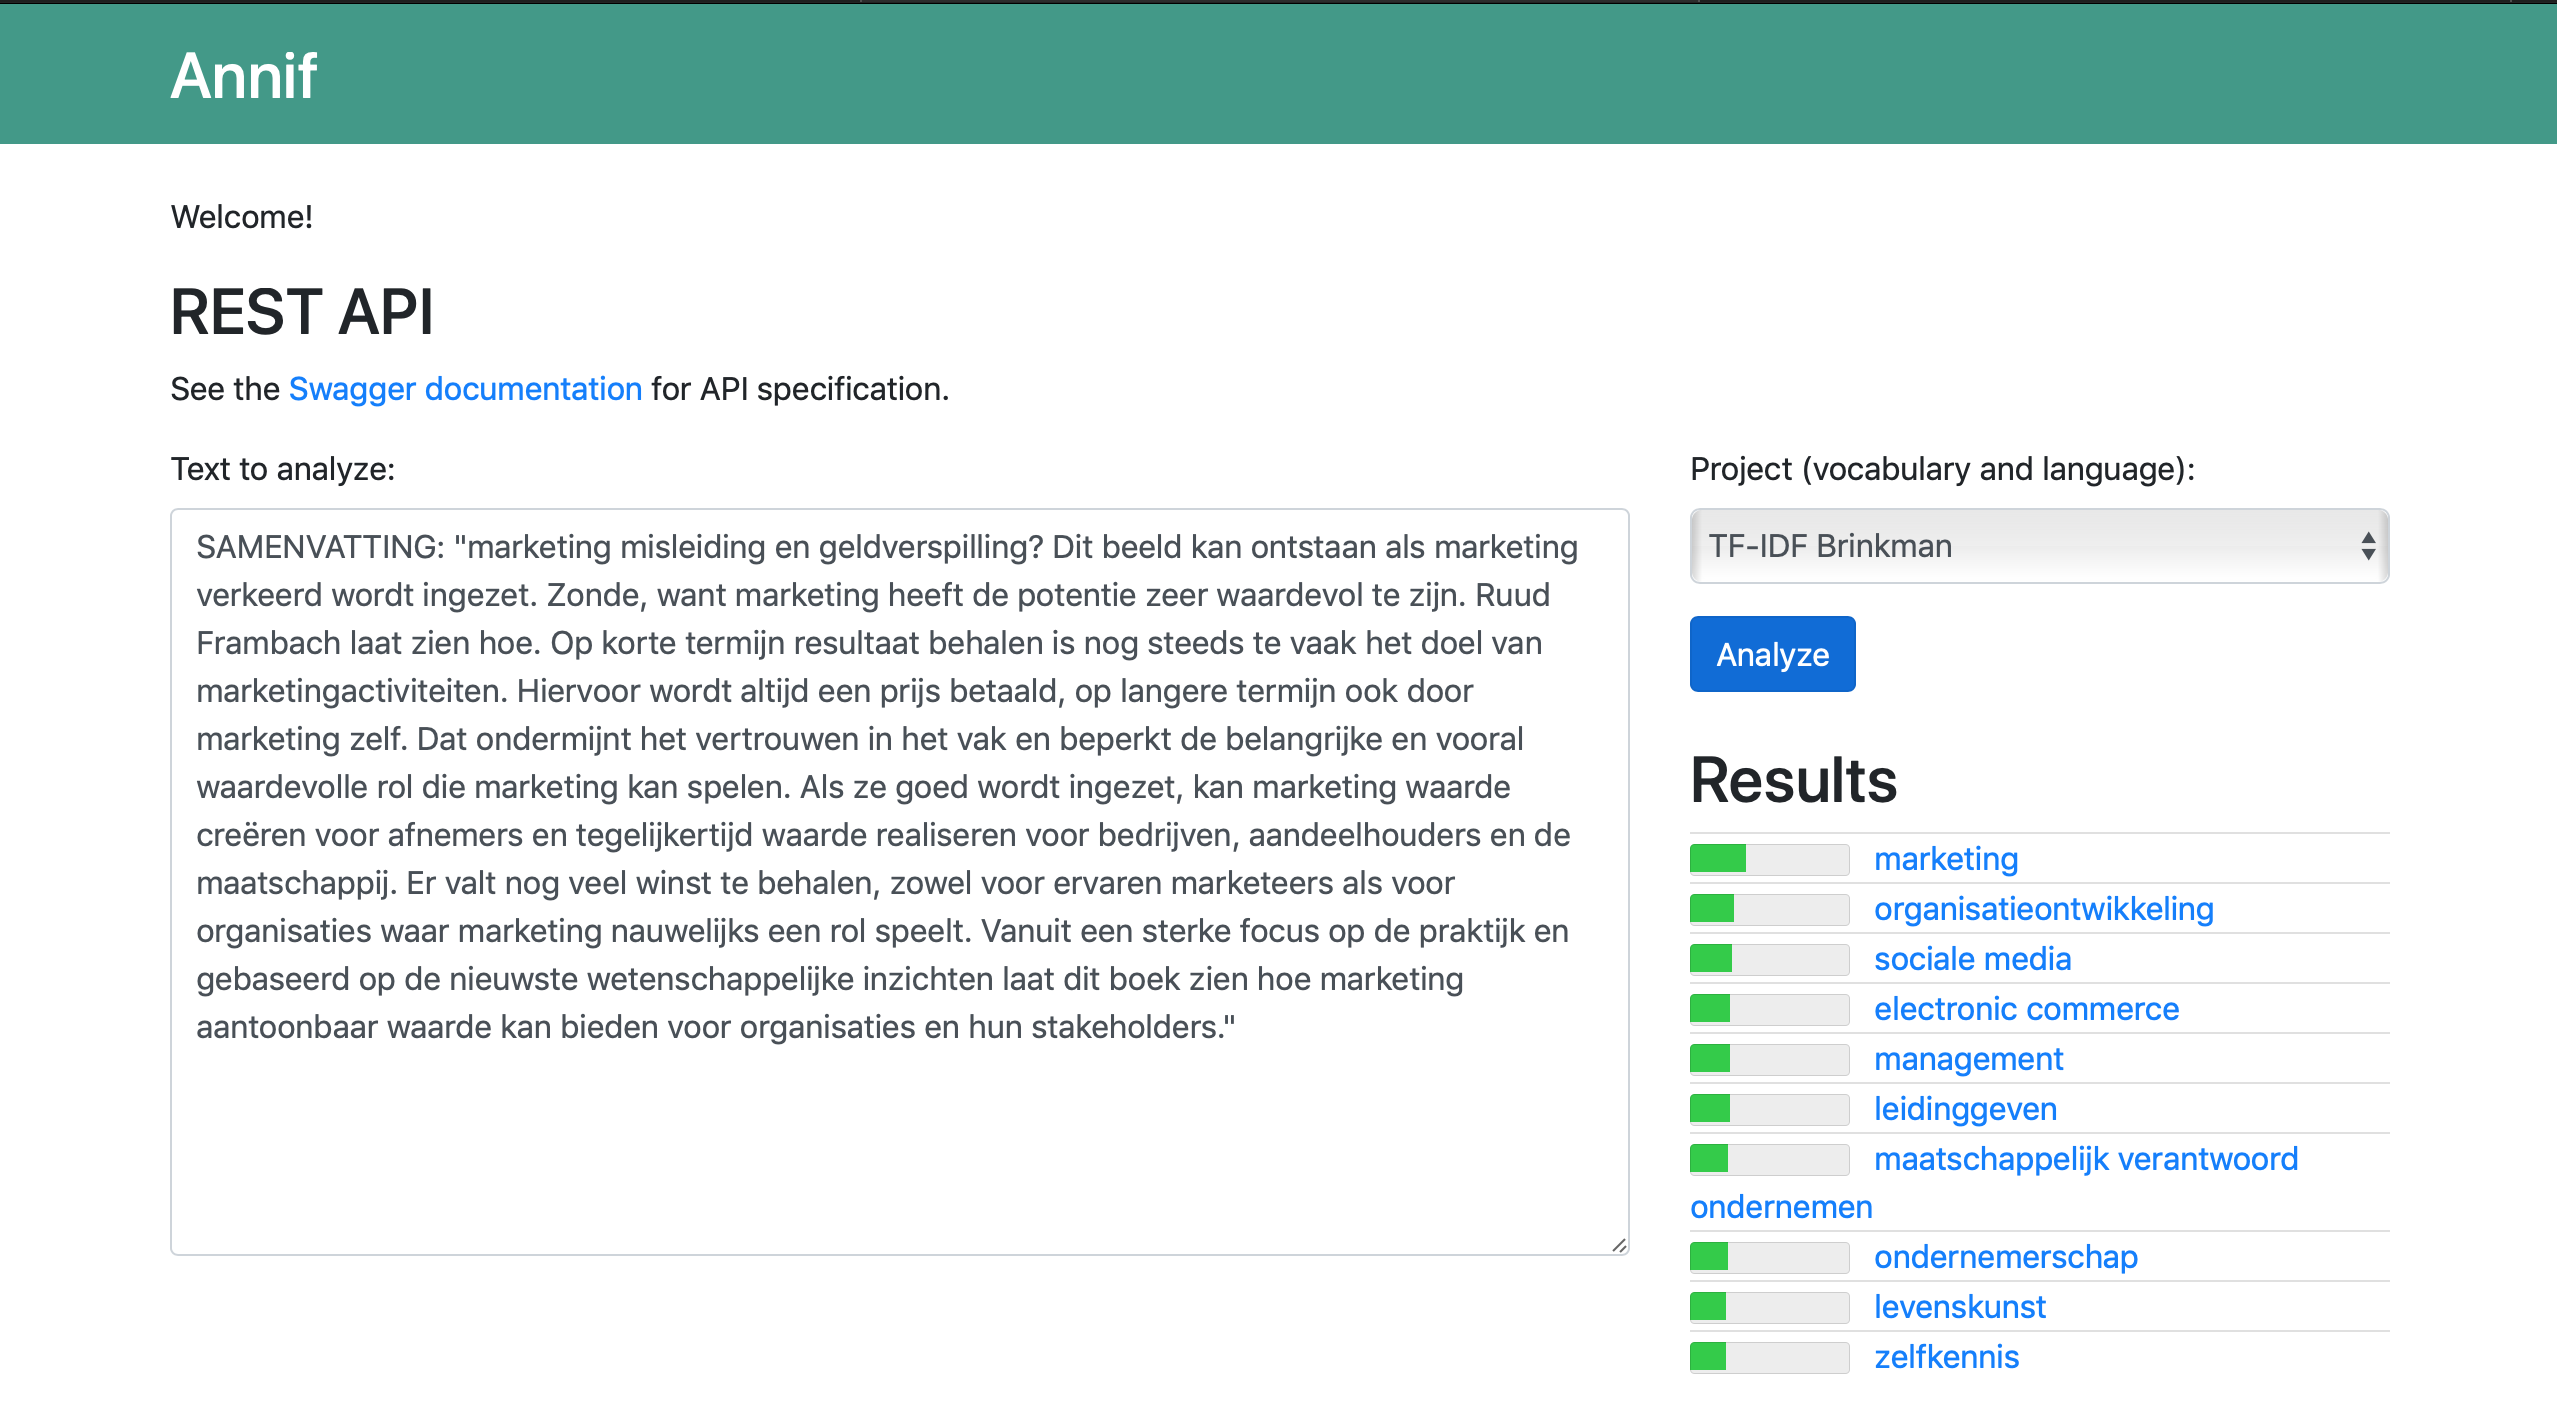
\includegraphics[width=150mm, scale=0.4]{7BBD85895892414FC9DD9978C35B6B14.png}

Bijbehorende toegekende Brinkman term: \\
\texttt{<http://data.bibliotheken.nl/id/thes/p075661098>	marketing}

\subsection{SKOS (Simple Knowledge Organization System)}

\begin{itemize}
  \item \href{https://www.w3.org/TR/2005/WD-swbp-skos-core-guide-20051102/}{SKOS Core Guide}
  \item \href{https://www.w3.org/TR/2005/WD-swbp-skos-core-spec-20051102/}{SKOS Core Vocabulary}
\end{itemize}

SKOS is een toepassing van RDF. SKOS standaard is specifiek te gebruiken voor het vastleggen van een thesaurus, gecontroleerde vocabulair e.d. SKOS maakt o.a. gebruik van synoniemen (\texttt{altLabel}) van een term (\texttt{Concept}, \texttt{prefLabel}) en de hierargische relatie (\texttt{broader}, \texttt{narrower}) tussen termen in een thesaurus.\\*[2pt]

\noindent
\textbf{Voorbeeld snippet}

\begin{lstlisting}[language=xml]
  <skos:Concept rdf:about="http://www.yso.fi/onto/yso/p21272">
    <rdf:type rdf:resource="http://www.yso.fi/onto/yso-meta/Concept"/>
    <skos:altLabel xml:lang="en">leaf beetles</skos:altLabel>
    <skos:broader rdf:resource="http://www.yso.fi/onto/yso/p6734"/>
    <skos:closeMatch rdf:resource="http://id.loc.gov/authorities/subjects/sh85025443"/>
    <skos:exactMatch rdf:resource="http://www.yso.fi/onto/allars/Y37803"/>
    <skos:exactMatch rdf:resource="http://www.yso.fi/onto/koko/p57371"/>
    <skos:exactMatch rdf:resource="http://www.yso.fi/onto/ysa/Y158869"/>
    <skos:inScheme rdf:resource="http://www.yso.fi/onto/yso/"/>
    <skos:narrower rdf:resource="http://www.yso.fi/onto/yso/p21619"/>
    <skos:prefLabel xml:lang="en">Chrysomelidae</skos:prefLabel>
    <skos:prefLabel xml:lang="sv">bladbaggar</skos:prefLabel>
    <skos:prefLabel xml:lang="fi">lehtikuoriaiset</skos:prefLabel>
  </skos:Concept>
\end{lstlisting}

\subsection{Maui backend}

\href{https://github.com/NatLibFi/Annif/wiki/Backend%3A-Maui}{Maui backend Annif Github}

\begin{shaded}
\noindent
Brinkman turtle bestand:\quad \href{run:/Users/haighton_macbook/Desktop/Projects/KB/automatisch_onderwerp_ontsluiting/scripts/data/thes_000001.ttl}{\textbf{\textit{thes\_000001.ttl}}} \\
Brinkman download: \quad \quad
\href{/Users/haighton_macbook/Desktop/Projects/KB/brinkman_skos/data/brinkman_dl.txt}{\textbf{\textit{brinkman\_dl.txt}}}

\end{shaded}

\subsubsection{Installatie Maui backend}

Maui Server image geinstalleerd op Macbook Pro \href{https://github.com/NatLibFi/MauiServer/tree/dockerization#usage-with-docker}{via Docker 2.2.0.0}. \\
Server kon benaderd worden via browser (localhost). 


\subsubsection{Brinkman catalogus in SKOS formaat}

Maui werkt met thesauri in het SKOS formaat. De Brinkman is niet direct in deze vorm te krijgen, wel in naderende vorm. Ik heb via Rene Voorburg een oude uitdraai van de Brinkman catalogus gekregen in het turtle (.ttl) formaat. En via zijn script \url{https://github.com/renevoorburg/oai2linerec} een huidige versie proberen te downloaden. De download heb ik na een dag of twee gestopt.
\\*
Brinkman SKOS download m.b.v. script Rene. Start script:
\begin{lstlisting}
sh oai2linerec.sh -p dcx -s GGC-THES -o brinkman_skos_test.txt -b http://services.kb.nl/mdo/oai
\end{lstlisting}

De verkregen download heb ik eerst moeten opschonen, omdat er niet alleen Brinkman trefwoorden in staan; gedaan m.b.v. een code editor en reguliere expressies. Deze heb ik daarna m.b.v. \href{https://github.com/NatLibFi/Skosify}{Skosify} omgezet naar een voor Annif bruikbaar bestand (default settings).

Het turtle bestand heb ik ook met Skosify bewerkt, omdat de inhoud van het bestand gesorteerd was op parameter.

Beide bestanden gaven niet direct een foutmelding wanneer het \texttt{vocab} command gebruik in Annif om het bestand als thesaurus aan te geven. Maar het trainen van een model wilde niet starten. Wanneer er via de browser naar de parameters werd gekeken (json bestand op de achtergrond, te zien in browser) die Maui had kon worden gezien dat er nog geen thesaurus was opgegeven. 

Uiteindelijk besloten om eens een test te doen met de bijgevoegde SKOS (\textit{yso-skos-boethius.rdf}) van Annif en deze werd ook niet geaccepteerd. Dit is een indicatie dat het waarschijnlijk niet meteen aan de gemaakte Brinkman SKOS lag (wat mijn eerste gedachte was), maar er ergens anders iets fout zat (bv. installatie docker Maui Server).


\subsection{Actie punten}
\href{https://trello.com/b/Hy6Ol32K}{personal Trello board}

  \begin{todolist}
    \item[\done] Configuratie aanpassen, i.e. probeer simple analyzer.
    \item Probeer verschillende backends - bv ensemble approach.
    
    \begin{todolist}
      \item[\done] TF-IDF
      \item[\done] Fasttext
      \item Maui 
      \item[\done] Omikuji
      \item Ensembles
    \end{todolist}

    \item Ook titel data gebruiken naast de samenvatting.
    \begin{todolist}
        \item[\done] Dataset gemaakt \href{https://github.com/KBNLresearch/Annif_data_exp/blob/master/vocab2.zip}{ggc2}.
        \item Testen, vergelijken met uitkomsten ggc dataset, en uitkomsten documenteren. \textit{nog niet met alle backends getest. De backends die getest zijn blijken net iets beter te werken met titel data.}
        \item Test met weights: 2x titel in data gebruiken.
    \end{todolist}
    \item Documentatie! (die lees je nu)
    \item SKOS vocab + Maui backend - Brinkman als SKOS. \\ 
    \textit{[05-03-2020] Met Sara besproken om Maui even te parkeren.}
    \begin{todolist}
      \item Minimale eisen SKOS bestand voor Annif met Maui backend (moeten we onderstaande punten gaan uitzoeken?).
      \item[\done] Hulp vragen Rene Voorburg om SKOS te genereren via OAI-PMH (GGC\_THES) - zie zijn script op \url{https://github.com/renevoorburg/oai2linerec}.
      \item Omvormen verkregen 'SKOS' data naar daadwerkelijk SKOS-XML bestand. 
      \item[\wontfix] Evaluatie model per woord. (gaat Sara oppakken)
    \end{todolist}
    \item Tweak backends en optimaliseer ensembles.
    \item \href{https://github.com/NatLibFi/Annif/wiki/Achieving-good-results}{Idee m.b.t evaluatie model} \\
    Annif testen tegen 2 collectiespecialisten, ieder probeert een brinkmantrefwoord toe te wijzen, m.b.v. word2vec kijken of de termen dicht bij elkaar liggen (of andere methodes; onderzoeken!)?
  \end{todolist}

  
\subsubsection{Actiepunten voor voortzettten testen Maui backend}
\begin{todolist}
  \item Andere manier van installeren via Tomcat (zie \url{https://github.com/NatLibFi/Annif/wiki/Backend\%3A-Maui#setting-up-maui-server-using-tomcat})
  \item Verse install Annif - gelijk testen met door Annif bijgevoedge SKOS (zou inprincipe direct moeten werken).
  \item Ronald Cornelisen mailen m.b.t. Brinkman SKOS. data.bibliotheken.nl opgezet (extern)
\end{todolist}


\end{document}